% !TEX root =  master.tex
\section{Bezahlvorgang}

Wenn der Benutzer all seine Plätze ausgewählt hat und auch die Ermäßigungen angegeben hat, gelangt er zur nächsten Seite, auf der er weitere Daten eingeben muss.

\begin{figure}[ht]
	\centering
	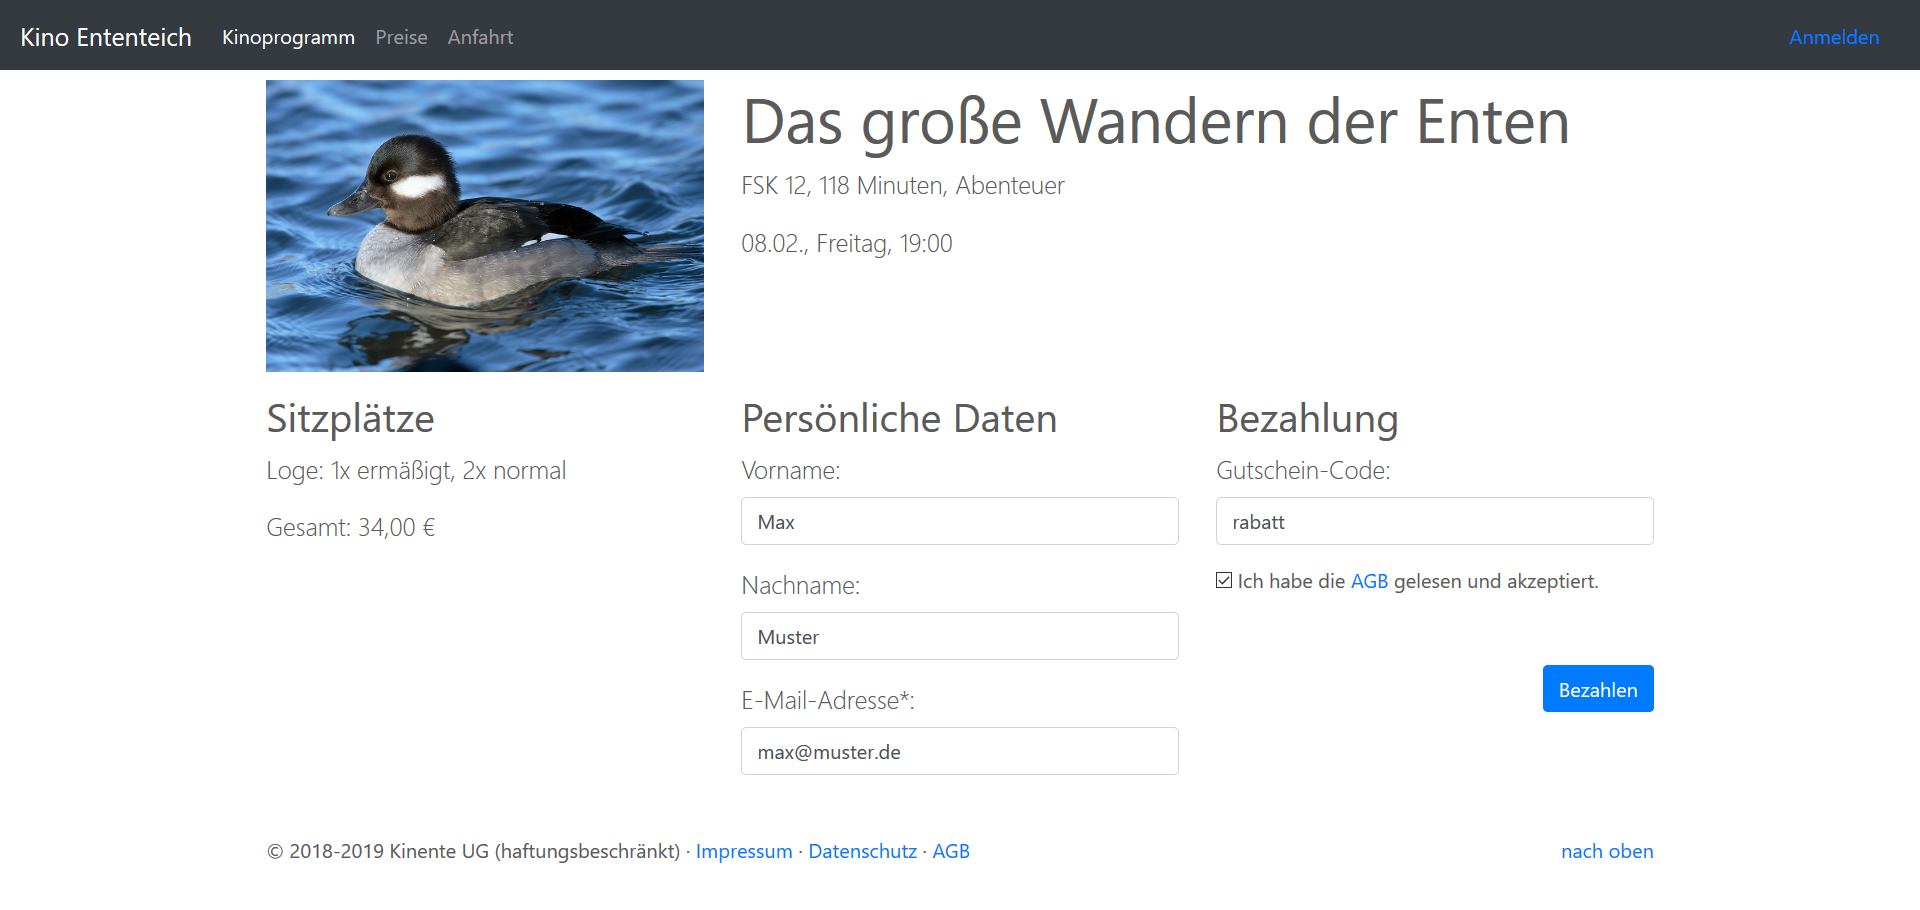
\includegraphics[width=0.95\textwidth]{img/screenshots/vorstellung03}
	\captionsetup{format=hang}
	\caption{Angabe weiterer Daten, die für den Buchungsvorgang relevant sind}
	\label{fig:vorstellung03}
\end{figure}

Die Daten zur Vorstellung, zu den ausgewählte Sitzplätzen, zu den Ermäßigungen und auch der Preis werden dabei über \acs{URL}-Parameter weitergegeben.
Auch wenn der Preis in diesem Fall redundant ist, so wird er trotzdem übergeben, um sich eine erneute Berechnung, die auch wieder eine weitere Kommunikation mit dem Back-End erfordern würde, zu ersparen.
Dies hat jedoch den Nachteil, dass der Benutzer Werte wie eben den Gesamtpreis theoretisch bei der Übergabe auf die nächste Seite ändern könnte und dann andere Werte angezeigt bekommt.
Dies betrifft jedoch nicht die Sicherheit des Systems, da alle Berechnungen und Überprüfungen zwangsläufig zumindest noch einmal im Back-End erfolgen müssen.
Am Beispiel des Preises würde dies bedeuten, dass der Benutzer zwar seine aktuelle Ansicht manipulieren kann, dennoch den korrekten Preis bezahlen muss.

Im oberen Bereich sieht der Benutzer nochmal allgemeine Informationen zur Vorstellung.
Des Weiteren erhält er eine Zusammenfassung zu seiner Sitzplatzauswahl mit dem Gesamtpreis.
Wenn sich der Benutzer entscheidet, die Sitzplätze verbindlich zu buchen, so wird im Hintergrund eine Nachricht an das Back-End gesendet.

Die Daten werden ähnlich wie beim Blocken eines Sitzplatzes in einem \acs{JSON}-Objekt gespeichert und mit einem \acs{AJAX}-Aufruf an das Back-End gesendet.

Im aktuellen Beispiel (siehe Abbildung \ref{fig:vorstellung02} und \ref{fig:vorstellung03}) würde sich dann folgendes \acs{JSON}-Objekt ergeben.

\begin{lstlisting}[language=JavaScript, caption={\acs{JSON}-Objekt für den Reservierungsvorgang}, label={lst:json_book}]
book = {paymentoption: "giftcard",
        verification: "rabatt",
        showId: 13,
        seats: [{id: 113, isReducedPrice: true},
                {id: 114, isReducedPrice: false},
                {id: 115, isReducedPrice: false}],
        customer: {firstname: "Max",
                   lastname: "Muster",
                   email: "max@muster.de"},
        sessiontoken: "TreevgQreNefpuUngHroreunhcgAvpugfTrznpug13"};
\end{lstlisting}

Neben den Informationen zur Vorstellung und den Sitzplätzen, wird auch noch die als Cookie gespeicherte Sitzungskennung mit angegeben.
Dies ist notwendig, damit eine Zuordnung zu den geblockten Sitzplätzen erfolgen kann.
Beim Auswählen des Sitzes wird der Sitzplatz für den Benutzer für eine gewisse Zeit geblockt.
Im Normalfall sind die Plätze beim Reservieren somit immer noch durch den Benutzer geblockt.
Durch die Angabe derselben Sitzungskennung, die auch beim Blocken verwendet wurde, ist es nun im möglich, dass im Back-End erkannt wird, dass der aktuelle Benutzer berechtigt ist, die geblockten Plätze zu reservieren.

Bei erfolgreicher Reservierung erhält man Informationen zur Reservierung, wie z.B. die Reservierungsnummer und die Tickets.
In diesem Fall kann auch die Bestätigung angezeigt werden, andernfalls erscheint eine Fehlermeldung.

Die Bestätigung enthält noch einmal alle Informationen zur Vorstellung, zur Anzahl der Sitzplätze und zum gezahlten Kaufpreis.
Unter einer kurzen Beschreibung zum weiteren Verlauf findet der Benutzer sein Ticket in Form eines \acs{QR-Code}s.
In diesem ist ein eindeutiger Verweis auf die Reservierung und somit auf alle Tickets gespeichert.
Der \acs{QR-Code} wird dabei unter Zuhilfenahme einer quelloffenen Bibliothek\footnote{\url{https://github.com/nayuki/QR-Code-generator}} erzeugt.

\begin{figure}[ht]
	\centering
	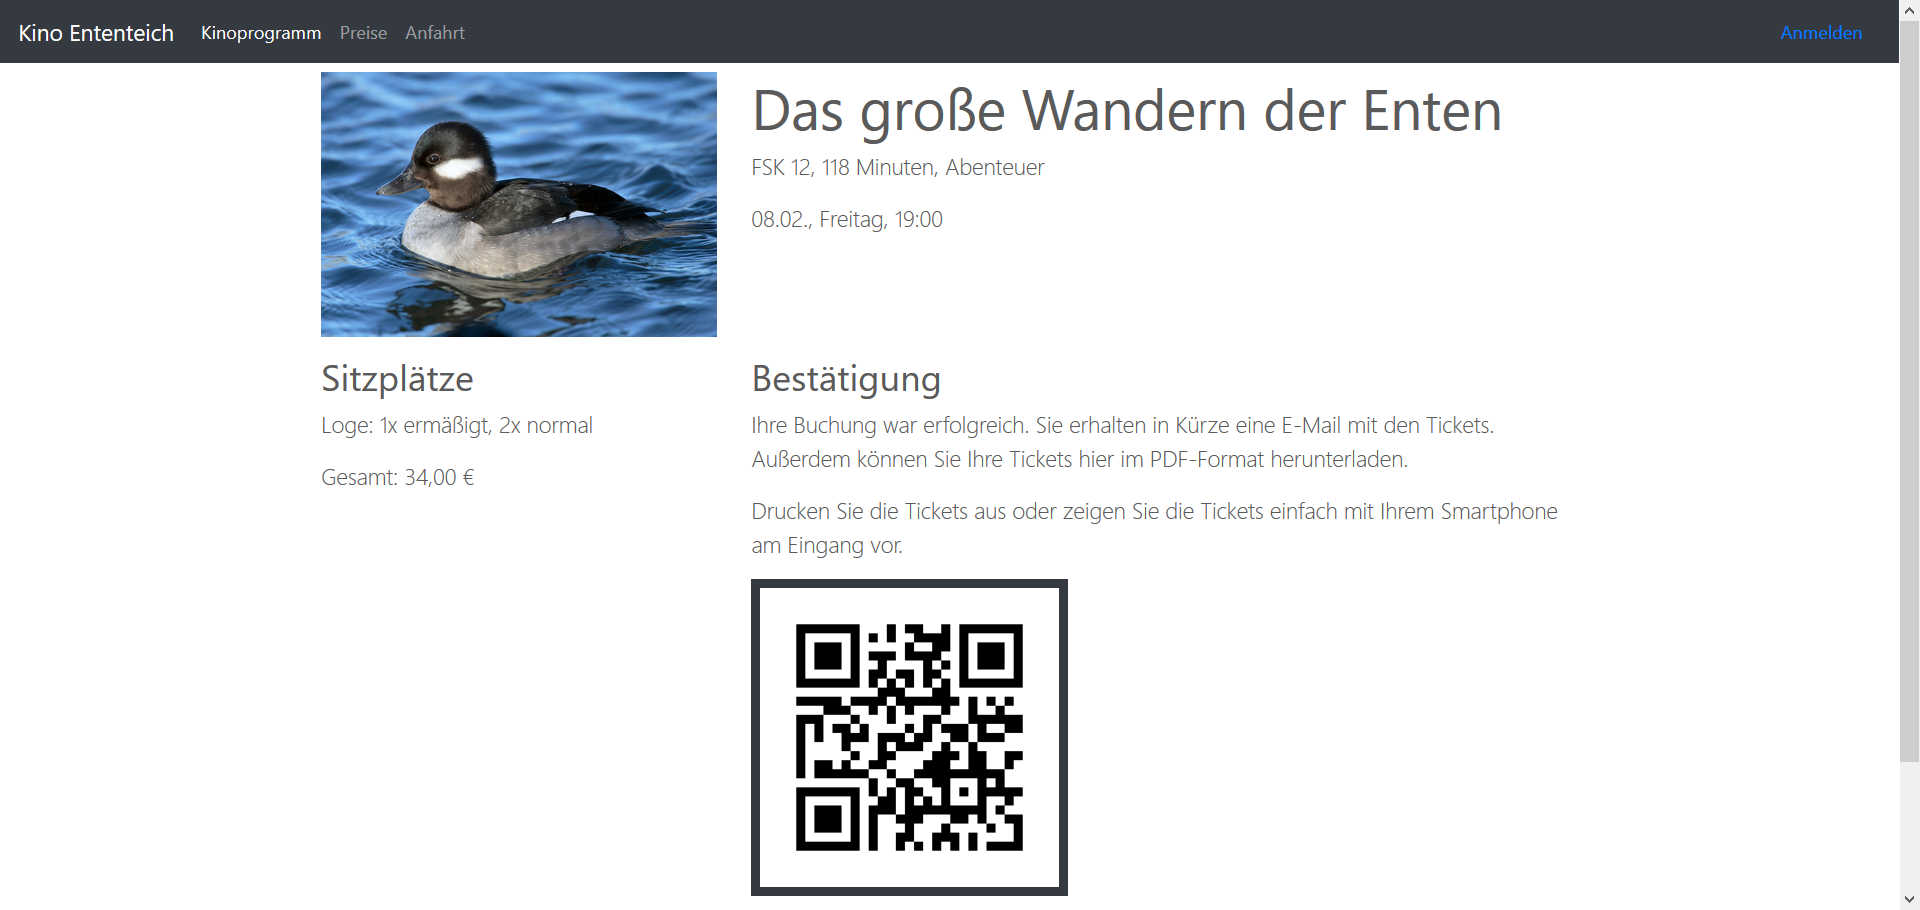
\includegraphics[width=0.98\textwidth]{img/screenshots/vorstellung04}
	\captionsetup{format=hang}
	\caption{Bestätigung einer Reservierung und Anzeige des \acs{QR-Code}s}
	\label{fig:vorstellung04}
\end{figure}

Im Kino kann an der Ticketkontrolle der \acs{QR-Code} gescannt und somit die Gültigkeit der Tickets überprüft werden.
Dadurch, dass ein \acs{QR-Code} für alle Tickets einer Reservierung steht, müssen sich die Benutzer, wenn sie mit mehreren Personen das Kino besuchen, keine Gedanken machen, wer welches Ticket erhält und die Tickets nicht untereinander verteilen. % TODO: move to design/planning?
